\part{Seminar 6 -- Fractional-Slot Concentrated-Windings
Synchronous Permanent Magnet Machines:
Opportunities and Challenges}

\makebox[.25\textwidth]{Martin Braquet}\makebox[.25\textwidth]{Alexandre Buset}\makebox[.25\textwidth]{Gilles Precup}\makebox[.25\textwidth]{Grégoire van Oldeneel}

\section{Introduction and reminders}
We all know synchronous machines (reminder just after ;) ). During the last seminaries we were focused on the modelling of all kind of electrical machines and perhaps you believe we were pretty well through with the subject. In fact, synchronous machines have still many unexplored opportunities.

One of them is the FSCW (Fractional Slot Permanent Concentrated Windings) with permanent magnets.


The synchronous machine is composed of a stator (cf. Figure \ref{fig:SMrotor}) containing the windings, and a rotor (either with permanent magnets or with dc supplied windings). The stator windings are typically supplied with alternative current inducing a rotating magnetic field. The rotor try to align itself with the stator rotating field. As a result, the rotor rotates synchronously with the rotor, which is called \textit{synchronous speed}:
\begin{equation}
    \omega_{sync} = \frac{\omega_{network}}{n_{pair\_of\_poles}}
\end{equation}

\begin{figure}[H]
    \begin{minipage}{0.49 \textwidth}
    \centering
        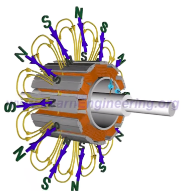
\includegraphics[scale = 0.50]{SMrotor.png}
        \caption{Synchronous machine: rotor}
        \label{fig:SMrotor}
    \end{minipage}
    \begin{minipage}{0.49 \textwidth}
        \centering
        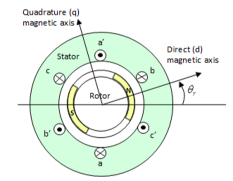
\includegraphics[scale=0.50]{SMmodel.png}
        \caption{Synchronous machine: model}
        \label{fig:SMmodel}
    \end{minipage}
\end{figure}

\section{Design of an FSCW machine}

What about the stator winding? Several designs exist. Here is just a first sight of the different existing configurations. The two above are classical synchronous machine, as we studied last year. The 2 below are concentrated windings. Those are the case studied.

\begin{figure}[H]
    \centering
    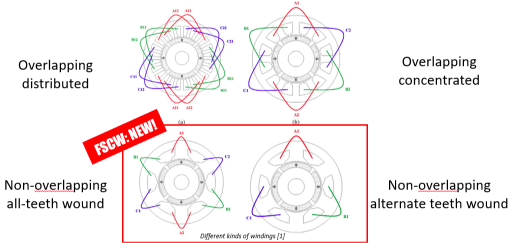
\includegraphics[scale=0.5]{SM.png}
    \caption{Kinds of synchronous machine design.}
    \label{fig:SM}
\end{figure}

Figure \ref{fig:SMarbre} clarifies the classification of the stator windings: on one hand, we have overlapping, and the windings could be concentrated or not concentrated; on the other hand, we have non-overlapping windings, which are concentrated, and we can distinguish all teeth wound from alternate teeth wound (illustrated on Figure \ref{fig:SM}). That’s we will study. As you can notice it, we can characterise the machine by a factor: the \textbf{number of slots per pole per phase}, defined as:
\begin{equation}
    S_{pp} = \frac{S}{2 \cdot p \cdot m}
\end{equation}
with:
\begin{itemize}
    \item $S$, the number of slots
    \item $p$, the number of pole pairs
    \item $m$, the number of phases 
\end{itemize}
In ‘classical’ machine, it’s always above or equal to one. For the FSCW, saying it roughly, we have less slots.  

\begin{figure}[H]
    \centering
    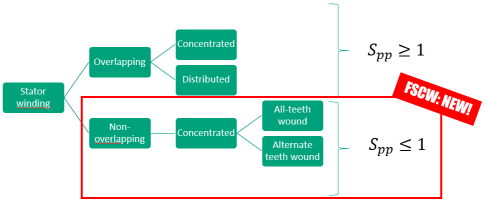
\includegraphics[scale=0.5]{SMarbre.png}
    \caption{Characterisation of the different synchronous machines.}
    \label{fig:SMarbre}
\end{figure}


\section{Working principle}
In order to understand the working principle of this machine, we will begin by looking at the magnetic field in the airgap of the machine induced by the stator. To do this, we will make some assumptions :
\begin{itemize}
    \item Smooth airgap (no salience)
    \item Stator winding replaced by conductor at the interface
    \item Small airgap compared to the radius $\Rightarrow$ magnetic field supposed purely radial
\end{itemize}
Then using the Ampere's Law of equation \ref{ampere_law}, we can compute the magentic field $\vec{H}$ in the airgap :
\begin{equation} \label{ampere_law}
    \oint \vec{H} \cdot \vec{dl} = N \cdot i
\end{equation}

\subsection{Magnetomotive Force}
\subsubsection{Overlapping Concentrated Winding}
An example of an overlapping concentrated winding machine (here a 12-slots 4-poles 3-phases machine) is shown in Figure \ref{12s4p3p}. In order to compute the magnetic field for the whole machine, we will first study the magnetic field induced by one phase as it is illustrated in Figure \ref{12s4p3p_1p} then generalise to the whole machine.

\begin{figure}[H]
    \begin{minipage}{.45 \textwidth }
        \centering
        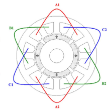
\includegraphics[scale=0.6]{scheme_winding.png}
        \caption{Winding of a 12-slots 4-poles 3-phases machine}
        \label{12s4p3p}
    \end{minipage}
    \begin{minipage}{.45 \textwidth }
        \centering
        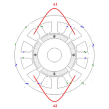
\includegraphics[scale=0.6]{scheme_winding_onephase.png}
        \caption{One phase of a 12-slots 4-poles 3-phases machine}
        \label{12s4p3p_1p}
    \end{minipage}
\end{figure}

The magnetic field of one phase is easily computed by using the exact same method used in the course LELEC1310. The Figure \ref{12s4p3p_1p_mmf} shows the magnetic field obtained for one phase. Figure \ref{12s4p3p_3p_mmf} presents the magnetic field when the 3 phases are combined. When using 3 phases, we need to pay attention to 2 things : 
\begin{itemize}
    \item The mechanical phase shift : $\theta_{mec}=\frac{360\degree}{p \cdot m}$ 
    \item The electrical phase shift : (0\degree , 120\degree , 240\degree) which correspond to coefficients equal to (0, $\frac{1}{2}$, $\frac{-1}{2}$)
\end{itemize}

\begin{figure}[H]
    \begin{minipage}{.45 \textwidth }
        \centering
        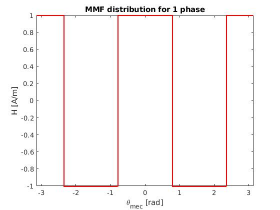
\includegraphics[scale=0.33]{mmf_one_phase.png}
        \caption{MMF distribution when considering only one phase}
        \label{12s4p3p_1p_mmf}
    \end{minipage}
    \begin{minipage}{.45 \textwidth }
        \centering
        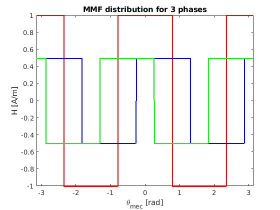
\includegraphics[scale=0.33]{mmf_3phases.png}
        \caption{MMF distribution when considering 3 phases}
        \label{12s4p3p_3p_mmf}
    \end{minipage}
\end{figure}

Finally, we can look at the sum of the contribution of the 3 phases and also the Fourier series of this sum as it is done in the Figure \ref{mmf_fourier_over_concentrated}
\begin{figure}[H]
    \centering
    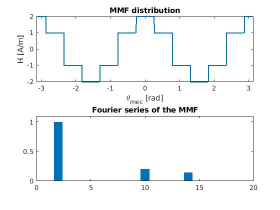
\includegraphics[scale = 0.45]{over_concentrated.png}
    \caption{MMF distribution and it's Fourier series of an overlapping concentrated machine}
    \label{mmf_fourier_over_concentrated}
\end{figure}

\subsubsection{Overlapping Distributed winding}
An example of an overlapping distributed winding machine (here a 24-slots 4-poles 3-phases machine) is shown in Figure \ref{24s4p3p}. The main difference with an overlapping concentrated winding is that instead of having $n$ wires in a single slot, the wires will be split into 2 consecutive slots with $\frac{n}{2}$ wires each. The method to compute the MMF distribution of the machine is exactly the same as described above so it won't be re-explained. The MMF and it's Fourier series is shown in the Figure \ref{mmf_fourier_over_distributed}.

\begin{figure}[H]
    \begin{minipage}{.45 \textwidth }
        \centering
        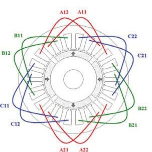
\includegraphics[scale=0.38]{scheme_over_distri.png}
        \caption{Winding of a 24-slots 4-poles 3-phases machine}
        \label{24s4p3p}
    \end{minipage}
    \begin{minipage}{.45 \textwidth }
        \centering
        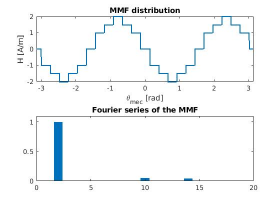
\includegraphics[scale=0.3]{distri.png}
        \caption{MMF distribution and it's Fourier series of an overlapping distributed machine}
        \label{mmf_fourier_over_distributed}
    \end{minipage}
\end{figure}

\subsubsection{Non-overlapping all-teeth wound winding}
An example of a non-overlapping all-teeth wound winding machine (here a 6-slots 4-poles 3-phases machine) is shown in Figure \ref{6s4p3p_all}. We can see that the winding do not overlap with each other anymore but there is 2 different windings in each slot. Even tough the configuration is different this still doesn't change the way we can compute the MMF distribution and it's Fourier series. The results are shown in the Figure \ref{mmf_fourier_nonover_all}.

\begin{figure}[H]
    \begin{minipage}{.45 \textwidth }
        \centering
        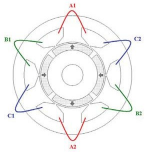
\includegraphics[scale=0.38]{scheme_conc_all.png}
        \caption{Winding of a 6-slots 4-poles 3-phases non-overlapping all-teeth wound machine}
        \label{6s4p3p_all}
    \end{minipage}
    \begin{minipage}{.45 \textwidth }
        \centering
        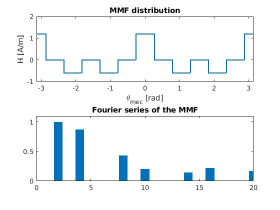
\includegraphics[scale=0.35]{all_teeth.png}
        \caption{MMF distribution and it's Fourier series of an non-overlapping all-teeth wound winding machine}
        \label{mmf_fourier_nonover_all}
    \end{minipage}
\end{figure}

\subsubsection{Non-overlapping alternate teeth wound winding}
An example of a non-overlapping alternate teeth wound winding machine (here a 6-slots 4-poles 3-phases machine) is shown in Figure \ref{6s4p3p_alternate}. In this configuration, the winding still do not overlap with each other but there is one more subtlety which is that there is only one winding in each slot. Once again, the computation of the MMF distribution and it's Fourier series is still the same. The result is shown in the Figure \ref{mmf_fourier_nonover_alternate}.

\begin{figure}[H]
    \begin{minipage}{.45 \textwidth }
        \centering
        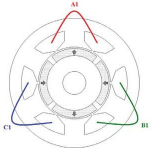
\includegraphics[scale=0.38]{scheme_conc_alternate.png}
        \caption{Winding of a 6-slots 4-poles 3-phases non-overlapping alternate teeth wound machine}
        \label{6s4p3p_alternate}
    \end{minipage}
    \begin{minipage}{.45 \textwidth }
        \centering
        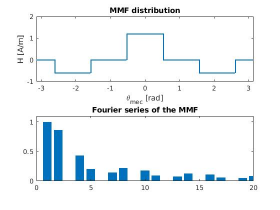
\includegraphics[scale=0.3]{nonover_alternate.png}
        \caption{MMF distribution and it's Fourier series of an non-overlapping alternate teeth wound winding machine}
        \label{mmf_fourier_nonover_alternate}
    \end{minipage}
\end{figure}

\subsection{Comparison of the different windings}\label{section_working_principle}
\subsubsection{Concentrated VS distributed}
As it was explain in the course LELEC1310, distributing the winding in an overlapping configuration allows to have a MMF distribution closer to a sine waveform and reduce the amplitude of higher order harmonics (we will see that it is useful as it decreases the losses). The difference is shown in the Figure \ref{comp_conc_distri}.

\begin{figure}[H]
    \centering
    \begin{subfigure}{0.45 \textwidth}
     \centering 
     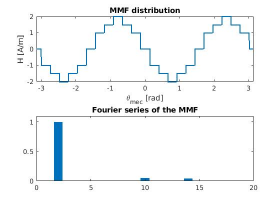
\includegraphics[scale=0.35]{distri.png}
     \caption{Distributed}
    \end{subfigure}
  \hspace{8pt}
    \begin{subfigure}{0.45\textwidth}
     \centering 
     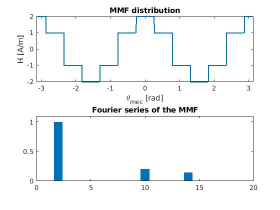
\includegraphics[scale=0.35]{over_concentrated.png}
     \caption{Concentrated}
    \end{subfigure}
    \caption{Comparison between overlapping concentrated and distributed winding}
    \label{comp_conc_distri}
\end{figure}

\subsubsection{Overlapping VS non-overlapping}
We can also compare overlapping and non-overlapping winding as it is done in the Figure \ref{comp_over_nonover}. It is obvious when we look at the MMF distribution of a non-overlapping winding in Figure \ref{comp_nonover} that we cannot clearly identify a spatial frequency as we are able to do in the Figure \ref{comp_over} for an overlapping winding. That is why it is interesting to also look at the Fourier series of this MMF distribution. We can see that there is 2 harmonics that dominates the first and the second harmonics. We can also note that even though the other harmonics have smaller amplitude, they not negligible compared to the main harmonics as it was the case for overlapping winding.

\begin{figure}[H]
    \centering
    \begin{subfigure}{0.45 \textwidth}
     \centering 
     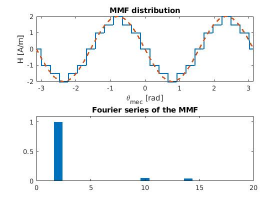
\includegraphics[scale=0.35]{distri_comparison_sine.png}
     \caption{Overlapping distributed}
     \label{comp_over}
    \end{subfigure}
    \begin{subfigure}{0.45\textwidth}
     \centering 
     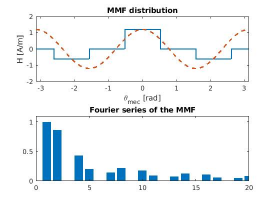
\includegraphics[scale=0.35]{allteeth_comparison_sine.png}
     \caption{Non-overlapping alternate teeth wound}
     \label{comp_nonover}
    \end{subfigure}
    \caption{Comparison between overlapping and non-overlapping winding}
    \label{comp_over_nonover}
\end{figure}

\subsubsection{In summary}
What is important to remember is that :
\begin{itemize}
    \item Overlapping winding has a MMF distribution close to a sine waveform and distributing the winding allows to have a purer waveform and reduce the amplitude of higher order harmonics
    \item Non-overlapping winding has a MMF distribution with a richer harmonic content so we need to use a Fourier series to identify the main harmonics. The amplitude of higher order harmonics is a lot more large than for overlapping winding.
\end{itemize}

\section{Design and analysis}

To produce the best machine, we want:

\begin{itemize}
    \item a high torque with low ripple: this implies reducing EMF harmonic distortion and the cogging torque
    \item a high efficiency: by maximizing the EMF
\end{itemize}

To reach these objectives, we can play with several parameters: the Slot/pole combination and the design of the stator windings.

\subsection{EMF optimisation}

The winding factor $k_w$ is the figure of merit (key performance) of the windings. It corresponds to the

"\textit{Ratio of flux linked by that winding compared to flux that would have been linked by a single-layer
full-pitch non-skewed integer-slot winding with the same number of turns and one single slot per
pole per phase.}"

Thus, maximizing $k_w$ aims at improving the RMS generated voltage in the 3-phase AC machines to minimize
the harmonics of the torque and the output voltage. This factor is splitted in three factors: $ k_w = k_d k_p k_s$.

\paragraph{Distribution factor $k_d$}

“\textit{The winding coils of each phase are distributed in a number of slots. Since the emf induced in different slots are not
in phase, their phasor sum is less than their numerical sum.}”

It is less than 1 for distributed windings, and equal to 1 for concentrated windings.

\[
    k_d = \frac{"\textrm{EMF with distributed windings}"}{"\textrm{EMF with concentrated windings}"} = \frac{\sin\left(\frac{\pi}{2mp}\right)}{\frac{S}{2mp}\sin(\pi/S)}
\]

\paragraph{Pitch factor $k_p$}

“\textit{The windings are often not fully pitched, i.e. the individual turns are reduced in order to decrease the length
of the end-turns and do not cover a full pole-pitch.}”

It highlights the fact that the windings do not catch all the flux available by the magnets.

\begin{enumerate}
    \item \textbf{Short} pitched coil, the phase angle between the induced emf of two opposite coil sides is less than 180°
(electrical).
    \item \textbf{Full} pitched coil: the phase angle between the induced emf of two coil sides is exactly 180° (electrical).
\end{enumerate}

\[
    k_p = \frac{"\textrm{EMF of short pitched coil}"}{"\textrm{EMF of full pitched coil}"} = \cos(\alpha/2)
\]
where $180-\alpha$ is the coil span: distance between the two sides of a coil.

\paragraph{Skew factor $k_s$}

“\textit{The windings (or the magnets) are angularly twisted in order to reduce the winding factor
harmonics introduced by the slotting of the stator, but it results in an angular spread and reduced emf.}”

It highlights the fact that the windings are not parallel to the magnets at the rotor.

\[
    k_s = \frac{\sin\left(\frac{z\pi p}{S}\right)}{\frac{z\pi p}{S}}
\]
where $z$ is the skew in number of slots, $p$ is the number of pole pairs, and $S$ is the number of slots.

\begin{itemize}
    \item \textbf{Advantage}: it reduces the preferential rotor position, thus the cogging torque and finally the torque ripple.
    \item \textbf{Drawback}: it also reduces the average torque (the useful one).
\end{itemize}

Thus, maximizing the EMF means maximizing
\[
    k_w = \frac{\sin\left(\frac{\pi}{2mp}\right)}{\frac{S}{2mp}\sin(\pi/S)} \cos(\alpha/2) \frac{\sin\left(\frac{z\pi p}{S}\right)}{\frac{z\pi p}{S}}
\]

We note that we can play with 4 parameters: \begin{itemize}
    \item $p$: number of pole pairs
    \item $S$: number of slots
    \item $\alpha$: related to the coil span
    \item $z$: skew
\end{itemize}
but we usually change the two first ones and analyse them in a 2D table (as shown in Figure \ref{fig:kw}).

\begin{figure}[H]
    \centering
    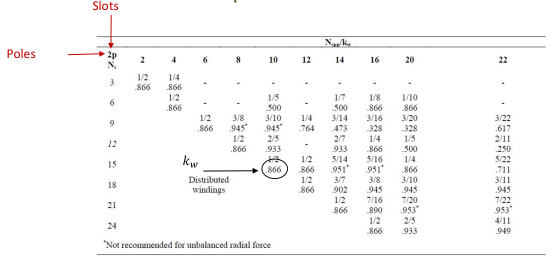
\includegraphics[width=0.6\textwidth]{kw.png}
    \caption{$S_{pp}/k_w$ for different slots and poles combinations}
    \label{fig:kw}
\end{figure}

\subsection{Torque ripple optimisation}

A torque ripple is introduced by

\begin{itemize}
    \item High harmonic content of the EMF
    \item The cogging torque: we have to minimize it because it is nul in average
\end{itemize}

\paragraph{Cogging torque ripple optimisation}

In overlapping windings, there is a non negligible cogging torque due to the preferential rotor position.

In FSCW: the different number of rotor/stator poles implies that
\begin{itemize}
    \item there is no preferential position of the rotor (low cogging torque)
    \item the number of slots at the stator must be higher and not a multiple of the number of rotor poles.
\end{itemize}

We want to reach a low cogging torque.
Knowing that "\textit{The number of cogging periods per rotor
revolution is given by the least common
multiple (LCM) of the pole and slot number}", this means we need a high cogging frequency to have a small amplitude of the cogging torque. This ends up with a large Least Common Multiple between $S$ and $2p$ (LCM($S,2p$)).

\paragraph{Cooking recipes}

\textit{Note that this part is a bonus for the interested reader.}

It also exists some cooking recipes to design the windings: e.g. the star of slots. We analyse an example for a 3-phase 12-slot 10-pole machine:



\begin{itemize}
    \item The star of slots is divided into $2m = 6$ sectors.
    \item Since $GCD(S,p) = GCD(12,5) = 12$ is even, the number of spokes in the positive sector is the same as the number of spokes in the negative sector.
    \item Divide the slots such that they are numbered 2 by 2, and assign a phase to each slot.
\end{itemize}

\section{High-power density}

The question is now: how to achieve high power density, which means the higher power transfer for the smallest machine volume?


\begin{figure}[H]
    \centering
    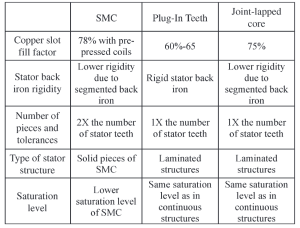
\includegraphics[width=0.4\textwidth]{HPDtable.png}
    \caption{Manufacturing techniques and their characteristics (coming from the paper)}
    \label{fig:HPD}
\end{figure}

The table (Figure \ref{fig:HPD}) sums up the main differences between the different manufacturing techniques. Clearly, if you have to choose, it depends on the purpose and on your budget. There are no perfect solution.

FSCW offers many advantages for the fabrication process. Once you know how many slot / poles you need, let's choose the manufacturing process.
For the design, we will keep in mind several criteria: 
\begin{itemize}
    \item Increase the \textbf{copper slot fill factor}\footnote{It’s an indicator which allows to know the quality of the winding. Greater is this factor, more powerful is your machine.}, defined as: $K_{cu,fill} = \frac{\text{Total copper area}}{\text{Total slot area}}$ (spare space into slots)
    \item Reduce the machine volume (evident reasons)
    \item Reduce copper volume (spare copper)
    \item Reduce manufacturing costs (spare time, above all: money)
\end{itemize}

\subsection{Joint-lapped core}
\begin{figure}[H]
    \begin{minipage}{0.49 \textwidth}
    \centering
        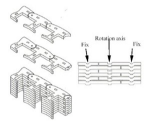
\includegraphics[scale = 0.50]{JLClink.png}
        \caption{Joint-lapped core: fabrication of the links.}
        \label{fig:JLClink}
    \end{minipage}
    \begin{minipage}{0.49 \textwidth}
        \centering
        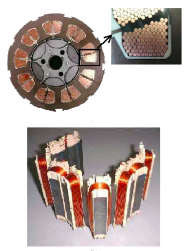
\includegraphics[scale=0.35]{JLCchain.png}
        \caption{Joint-lapped core: resulting chain.}
        \label{fig:JLCchain}
    \end{minipage}
\end{figure}
The first technique is the Joint-lapped core. It use the fact that the windings are not overlapped to easily mount them on segmented stator .
First, you laminate small component, you stack them (cf. Figure \ref{fig:JLClink}) and you assemble the links. Then you obtain a chain with teeth (cf. Figure \ref{fig:JLCchain}). Around each tooth, you can easily coil the copper wire, properly, avoiding to loose place. As a result, we can obtain really high copper slot fill factor. But as drawback, you obtain a lower rigidity.

\subsection{Plug-in teeth}

\begin{figure}[H]
    \centering
    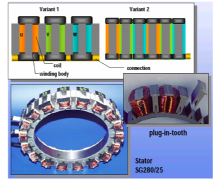
\includegraphics[width=0.4\textwidth]{PIT.png}
    \caption{Plug-in teeth: example}
    \label{fig:PIT}
\end{figure}

Second technique: Plug-in teeth. Here the stator is composed of one single rigid laminated iron piece with small tooth (cf. Figure \ref{fig:PIT}). Windings are coiled apart. Then you plug these small ring around the tooth and finally, you fix it with the e second part of the tooth. 
This technique allows to achieve quite high slot fill factor, while keeping a rigid stator.
The main part of the stator is laminated to reduce eddy current.

Thanks to concentrated windings, we can make each winding as a single part. To benefit from this design, each winding will be compressed. So, we reduce the winding volume,w e spare copper because the required wire is shorter (no right angle) and it is cheaper because easily manufactured. What about the tooth? As you could see, the tooth seems to be made all in one piece, like a iron bloc. But if it was the case, we would have lots of Eddy current losses. Fortunately, we have a alternative: using \textbf{Soft Magnetic Composite}.

\subsection{SMC: Soft Magnetic Composite}

\begin{figure}[H]
    \centering
    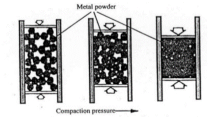
\includegraphics[width=0.4\textwidth]{SMC.png}
    \caption{Soft Magnetic composite}
    \label{fig:SMC}
\end{figure}

Basically, SMC is like small balls, mixed with resin and compressed. As a result, we obtain all kinds of desired forms with a high resistivity. Not only you can mould a teeth, but also it allows highly specific stator design, always with the aim to reduce the motor volume, spare copper, have a lighter part and reduce losses. On the manufacture point of view, it allows cheap mass production for big quantities. Unfortunately, the component are really brittle.

powder materials allows improvements over the lamination core with the respects of design freedom, low manufacturing cost, simple manufacturing processes, and low eddy current losses. 
On the electrical point of view, since the particles of the powder are insulated by the surface coating and adhesive used for composite bonding, the eddy current loss is much lower than in laminated steels, especially at higher frequencies, and the hysteresis loss becomes the dominant component of core loss. 
On the other hand, we dissipate less heat.


\section{Flux weakening}
\subsection{Problem}

\begin{figure}[H]
    \centering
    \begin{circuitikz} 
        \draw (0,0) to[V, v=$\omega_{em}\psi_{d0}$] (0,3) to [R, i>^=$\bar{I_s}$, l=$R_s$] (3,3);
        \draw (2.5,3) to [L, l=$j\omega_{em}L_{os}$] (5,3);
        \draw (5,0) to[V, v_=$\bar{V}_{s}$] (5,3);
        \draw (5,0) -- (0,0);
    \end{circuitikz}
    \caption{Simplified electrical circuit of a synchronous machine}
    \label{fig:circuit_SM}
\end{figure}

By analysing the simplified electrical circuit of a synchronous machine (cf. \autoref{fig:circuit_SM}), we see that increase the speed of the machine, $\omega_{em}$, also increase the supply voltage needed, $V_s$.

\begin{figure}[H]
    \centering
    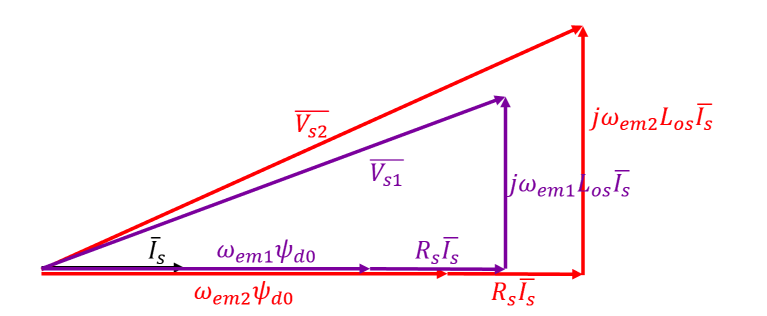
\includegraphics[scale=0.7]{phasor_diag.png}
    \caption{Phasor diagram of the simplified synchronous machine}
    \label{fig:diag_SM}
\end{figure}

As you can see on \autoref{fig:diag_SM},

\begin{equation}
    \omega_{em1} < \omega_{em2} \Rightarrow V_{s1} < V_{s2}
\end{equation}

Unfortunately, because of the power electronic that we use, we are limited in the voltage tension that we can provide. Therefore, we are also limited in the speed of the machine that we are able to reach.

The solution to this problem is the so called \textit{Flux weakening technique}. But first, we have to make a small reminder of LELEC2313.

\subsection{Reminder of LELEC2313: $d$ and $q$ equations}

We can write the system of equation which rule the dynamic of a permanent magnet synchronous machine. However, this system is very complex in the $abc$ system (3-$\phi$ system). 
\begin{itemize}
    \item The equations are all coupled together because the inductance matrix is full
    \item The currents will be changing rapidly, in steady-state, with the pulsation $p\omega_m$. So it will be very difficult to control.
\end{itemize}
The solution is to change the change the system of reference. We will so express the equations in the $dq$ system. This new system has the particularity of being a space vector system which turn with turn with the rotor. We are able of changing the system by using the Park (P) and Concordia (T) transformations (cf. \autoref{fig:sys_transf}).

\begin{figure}[H]
    \centering
    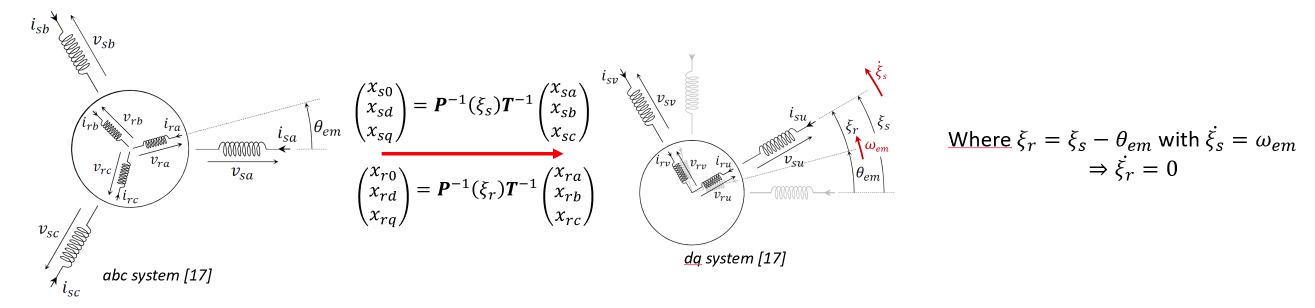
\includegraphics[scale=0.55]{park_concordia_transf.png}
    \caption{Transition from system $abc$ to system $dq$}
    \label{fig:sys_transf}
\end{figure}

The equation in the $dq$ system are the following:

\[
\left\{
\begin{array}{r c l}
     v_d &=& R_s i_d + L_d \frac{di_d}{dt} - \omega L_q i_q \\
     v_q &=& R_s i_q + L_q \frac{di_q}{dt} + \omega L_d i_d + \sqrt{\frac{3}{2}} \psi_0 \omega_m\\
     T_{em} &=& p[(L_d - L_q)i_q i_d + \sqrt{\frac{3}{2}} \psi_0 i_q]
\end{array}
\right.
\]

If we are working with permanent magnet synchronous machines (PMSM), because of the isotropy of the rotor, $L_d = L_q$. The electromotive torque may be rewrite:

\begin{equation}\label{eq:torque}
    T_{em} = \sqrt{\frac{3}{2}} \psi_0 i_q
\end{equation}

So the main idea of the control of a permanent magnet synchronous machine, is to keep the current $i_d$ equal to 0 because it produce no couple.

\subsection{Working principle}

\textit{"We will reduce the electromotive force by demagnetising the permanent magnet. To do this, we will create a supplementary negative flux component in the d-axis."}

To do this, we have in the linear case the expression of the flux:
\begin{equation}\label{eq:flux}
    \psi_d = L_d i_d
\end{equation}

So we will inject a negative $i_d$ current, in order to create a negative flux component in the d-axis. We can see it by an other way. Indeed, if we look at the $dq$ system of the PMSM. We see that in injecting a negative current $i_d$, we will decrease the $v_q$ component of the tension and so the supply tension itself.

\begin{figure}[H]
    \centering
    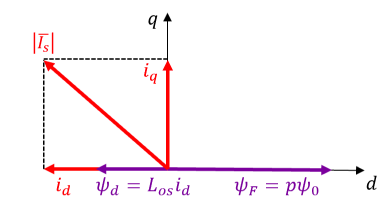
\includegraphics{injection.png}
    \caption{Representation of the injection of a negative flux component in the d-axis}
    \label{fig:injection}
\end{figure}

Unfortunately, again, we are limited in the maximal amplitude of the supply current. Yet, by injecting a negative $i_d$ current we have increase the amplitude of the supply current:
\begin{equation}
    \|\bar{I_s}\| =  \sqrt{i_d^2 + i_q^2}
\end{equation}
Hence, when we reach the current limit, to be able of increase the speed of the machine, we will have to reduce to $i_q$ current and so because of \autoref{eq:torque}, we will decrease the torque capability of the machine (cf. \autoref{fig:torq_capa}).

\begin{figure}[H]
    \centering
    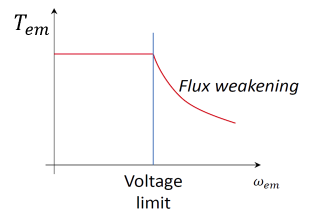
\includegraphics{torque_capa.png}
    \caption{Evolution of the torque capability of the machine with its speed}
    \label{fig:torq_capa}
\end{figure}

\subsection{Advantage of FSCW machines}

The main idea of the \textit{Flux weakening technique} is the inject the highest negative component in the d-axis with the smallest current $i_d$:
\begin{itemize}
    \item The highest negative component in the d-axis: In order minimize the supply voltage.
    \item The smallest current $i_d$: In order to minimize the losses of torque capability. 
\end{itemize}
And because of \autoref{eq:flux}, if we can increase $L_d$, we will inject more $\psi_d$ with less $i_d$. Yet:
\begin{equation}
    L_d = L_s - M_s
\end{equation}

And because of the leakage existing in the FSCW machines:
\begin{itemize}
    \item Harmonic leakage
    \item Slot leakage
\end{itemize}
The value of the mutual inductance of the stator, $M_s$, is very small compare to other kind of machines. So we have for the FSCW machine a much more Flux weakening capability (cf. \autoref{fig:comparison_torq_capa}). 

\begin{figure}[H]
    \centering
    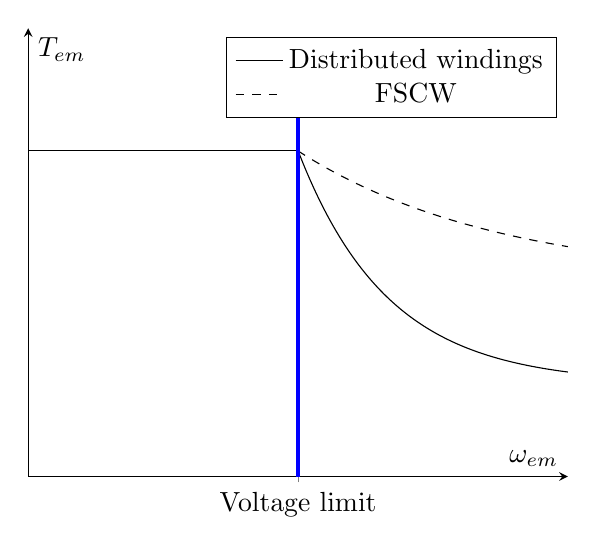
\begin{tikzpicture}
        \begin{axis}[
         clip=false,
         xmin=0,xmax=4,
         xlabel= $\omega_{em}$,
         ylabel=$T_{em}$,
         ymin=0,ymax=5.5,
         axis lines=middle,
         %axis x line=middle,
         %axis y line=left,
    %     axis x line=middle,
         xtick={2},
         xticklabels={Voltage limit},
         ytick={0},
         yticklabels={},
         legend entries={Distributed windings, FSCW}
         ]
          \addplot[domain=0:4,samples=200,black](0,4) -- (2,4);
          \addplot[domain=2:4, samples=200, black,dashed]{exp(-(x-2.7)/1.5)+2.4};
          \addplot[domain=2:4, samples=200, black]{exp(-1.5*(x-2.7))+1.14};
          \addplot[domain=0:4, samples=200, blue, very thick](2,0) -- (2,4.5); 
        \end{axis}
    \end{tikzpicture}
    \caption{Evolution of the torque capability of the machine with its speed in a FSCW machine vs in a distributed windings machine}
    \label{fig:comparison_torq_capa}
\end{figure}

\section{Rotor losses}
\subsection{Origins}
There is two main origins to rotor losses as it is depicted in Figure \ref{rotor_losses_origins}. The first one is due to air friction. This kind of losses happen only in high speed machine and won't be discussed any further here. The second source of losses is due to eddy currents. This source will be discussed in more details in the next section.
\begin{figure}[H]
    \centering
    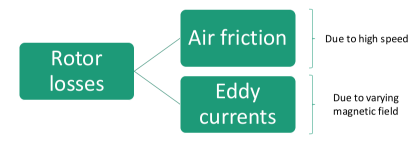
\includegraphics[scale=0.4]{rotor_losses_origins.png}
    \caption{Rotor losses origins}
    \label{rotor_losses_origins}
\end{figure}
\subsection{Eddy currents}
Eddy currents are generated by varying magnetic field. When the machine is rotating at the synchronous speed, the main harmonic does not generate any eddy currents in the rotor as both of them rotate synchronously. The problem is that there is a lot of harmonics content with non-overlapping concentrated winding as it was discussed in the section \ref{section_working_principle}. All this harmonics lead to the generation of eddy current and thus losses caused by Joule effect.

Another source of eddy current is the interaction with the teeth. This source is not taken into account into the computation of the MMF distribution as we made the hypothesis that we had a smooth airgap. In reality, teeth cause disturbances in the MMF distribution with a high order harmonics contents. This high order harmonics lead to more eddy current and more losses.

\begin{figure}[H]
    \centering
    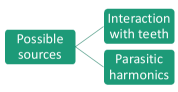
\includegraphics[scale=0.6]{eddy_current_origins.png}
    \caption{Eddy currents origins}
    \label{eddy_current_origins}
\end{figure}
\subsection{Drawback}
This losses will cause 2 major problems. The first one is that some power will be converted into thermal power instead of mechanical power. That means that the efficiency of the machine is reduced.

The other problem is also linked to the Joule losses. This losses will increase the temperature of the rotor. The problem is that the magnetic field generated by the magnet decreases as the temperature increases as it is shown in Figure \ref{magnet_field}. If we reach the Curie temperature, the magnet will be completely demagnetised and the machine is broken. Note that problem can arise sooner ! In practice, the magnet would be broken earlier because the magnetic field generated by the stator winding would change the magnetisation.

\begin{figure}[H]
    \centering
    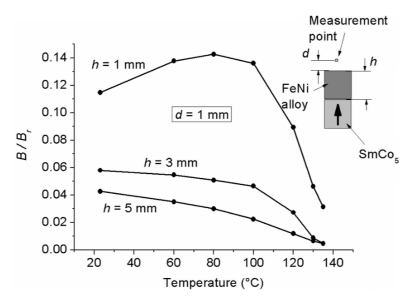
\includegraphics[scale=0.4]{magnet_field.png}
    \caption{Evolution of the magnet field in regard to temperature}
    \label{magnet_field}
\end{figure}

\subsection{Solutions}
We highlight 2 possible solutions in order to minimize the rotor losses. The first one is laminating the rotor in order to limit the circulating path of the eddy currents.

The second solution is to use a non-magnetic conducting sleeve. This sleeve allows to concentrate the joule losses at the surface of the rotor where it is easier to cool. It helps to prevent the overheating of the magnet. This sleeve can also be laminated in order to limit the circulating path of the eddy current and thus losses.

\section{Rotor design}
How to design your rotor? You have to minimize the losses, to easily dissipate the heat and finally, the most important, to maintain your magnets. Because at high speed, centrifugal effect can become really important. To maintain this magnets, you have 2 ways: 
glue them. But be careful: if the motor reach high temperature, the glue lose his stick capability (typically 120°C ).
The second possibility, more expensive: non-magnetic sleeve (made with Inconel steel, titanium or carbon composite). Then, eventually, you can add a copper coating: thanks to that, you concentrate your losses on the sleeve which is easier to cool.

\begin{figure}[H]
    \centering
    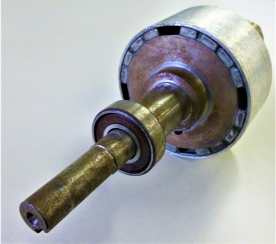
\includegraphics[scale=0.15]{Rotor.png}
    \caption{Rotor with permanent magnets and sleeve.}
    \label{fig:Rotor}
\end{figure}


\section{Parasitic effects}
The main drawback of the FSCW is its parasitic effects:
\begin{itemize}
    \item First source of parasitic effect is the high number of harmonics (cf. Figure \ref{fig:PEfourier}) of the magnetomotive force, generating unbalance tangential forces.
    \item The second problem is the asymmetrical coil distribution: as you can see, we obtain a quite strange distribution of the force in function of the electrical angle (cf. Figure \ref{fig:PE}).
\end{itemize}
As a result, the machine is affected by high vibrations and it generates noise.
It justifies why it is especially important to ensure a good maintain of the rotor permanent magnets.
\begin{figure}[H]
    \begin{minipage}{0.49 \textwidth}
        \centering
        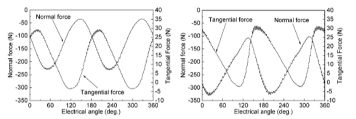
\includegraphics[scale=0.41]{PEtorqueripple.png}
        \caption{Parasitic effects: force distribution. Left: 8-poles/12-slots model; Right: 8-poles/9-slots mode.}
        \label{fig:PE}
    \end{minipage}
    \begin{minipage}{0.49 \textwidth}
        \centering
        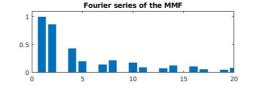
\includegraphics[scale=0.41]{PEfourier.png}
        \caption{Parasitic effects: harmonic content}
        \label{fig:PEfourier}
    \end{minipage}
\end{figure}

%\textcolor{red}{Je ne sais plus qui le faisait =)}


\section{IPM vs SPM machines}

Interior Permanent Magnets have their permanent magnets embedded into
the rotor itself. They are thus very mechanically robust, which enables them to reach very high speeds. There is less airgap because the air is replaced by metal (advantage).
The high magnetic saliencies generate a torque by magnetic and \textbf{reluctance}
torque components, thus the reluctant torque needs to be well designed in order to be positive.
Because the IPM machines are subject to recent research, these advantages are not clear yet.

Surface Permanent Magnets are mostly used, their magnets are fixed to the exterior of the rotor surface. This has a weaker mechanical strength and thus a lower maximum speed. The torque is only electrodynamic since the magnetic saliencies are limited.

\section{Fault tolerance}

\textit{"The fault tolerance of a system is its ability to pursue its function despite a partial failure."}

The fault tolerance is a key concept in electromechanical converters and especially for PM (permanent magnet) machines. Indeed, PM cannot be de-excited in case of failure. So these magnets may induce adverse effects. 

In electromechanical machines, there are 2 main types of failures:
\begin{itemize}
    \item A phase is short-circuited: Worst case because when cannot easily know the value of the current in the phase
    \item A phase is open-circuit: The current is equal to 0[A].
\end{itemize}
In the literature, we found certain criteria which can define the fault tolerance of electromechanical machines:
\begin{itemize}
    \item Isolation between phases: In order to avoid parasitic effect of the lost phase(s)
    \begin{itemize}
        \item Electric isolation
        \item Magnetic isolation
        \item Thermal isolation
        \item Physical isolation
    \end{itemize}
    \item Higher number of phases: Larger the number of phase is, smaller the impact of losing 1 phase will be.
    \item Implicit limitation of fault currents: Because of the Joule's effect, fault currents will produce heat and if this heat is not controlled, it can lead sever damages.
\end{itemize}
    
\subsection{In FSCW machines}
    
By construction, the concentrated winding machines have a better isolation between phases (electric, magnetic, thermal, physical).
\begin{figure}[H]
    \centering
    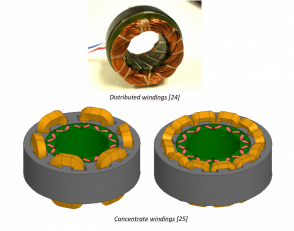
\includegraphics[scale=0.8]{fault_tol_C_vs_D.png}
    \caption{Representation of the difference between a concentrated winding machine and a distributed winding machine}
    \label{fig:fault_CvsD}
\end{figure}
So concentrated winding machines have really effective fault tolerance. Mainly the alternate teeth wound. 

\subsection{Control in fault tolerance}
The main idea is to supply the machine with new values of current in the remaining phases in order to keep the same torque:
\begin{equation}
    T_{ref} = \sum_{k=1}^n i_k \frac{d\psi_k}{dt}
\end{equation}
Where $i_k = 0$ for all the fault currents\footnote{So we consider here only phases which are open-circuit}. 

Then, we will find the optimal values of the currents by using a Lagrangian formulation. The constraints will be given in order to satisfy different configurations:
\begin{itemize}
    \item Non-sinusoidal currents
    \begin{itemize}
        \item Currents without a zero-valued sum
        \item Currents with a zero-valued sum
    \end{itemize}
    \item Sinusoidal currents
    \begin{itemize}
        \item Currents without a zero-valued sum
        \item Currents with a zero-valued sum
    \end{itemize}
\end{itemize}

\section{Commercial applications}
\begin{figure}[H]
    \begin{minipage}{0.49 \textwidth}
        \centering
        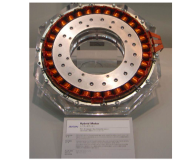
\includegraphics[scale=0.41]{CAtoyota.png}
        \caption{Toyota/Aisin Motor}
        \label{fig:CAtoyota}
    \end{minipage}
    \begin{minipage}{0.49 \textwidth}
        \centering
    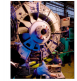
\includegraphics[scale=0.41]{CAship.png}
        \caption{Eigtheen-megawatt PM ship propulsion machine by DRS}
        \label{fig:CAship}
    \end{minipage}
\end{figure}
For the Toyota (cf. Figure \ref{fig:CAtoyota}), the constructor want a machine able to deliver high torque (so high copper slot fill factor), easy to manufacture. In this case, the segmented stator structure is used.

For the second one (cf. Figure \ref{fig:CAship}), such an application require high fault tolerance capability: even if a failure occur, the ship must be able to move forward. Thanks to its reliability, the motor is also used for aerospace and aircraft application. Perhaps you’re asking yourself: what about the parasitic effect, like torque ripple? Well in the case of heavy motors, inertia acts like a filter making the torque smoother.

\section{Conclusion}

FSCW machines have shown significant advantages but several drawbacks prevent it to replace all synchronous machine applications. It needs to be subjected to more research in the future in order to be a common synchronous machine available in more applications.

The main are positive characteristics are a high torque, a good flux weakening capability, a low cogging torque compared to other synchronous machines, a fault tolerance suitability, and low manufacturing costs.

The main drawbacks are their high harmonics contents (implying torque ripple) and the rotor losses.
